%!TEX program = xelatex
% 完整编译方法 1 pdflatex -> bibtex -> pdflatex -> pdflatex
% 完整编译方法 2: xelatex -> bibtex -> xelatex -> xelatex
\documentclass[lang=cn,11pt]{elegantpaper}

\title{A Network Embedding Augmented Collaborative Filtering Model For Recommendation}

\author{袁梦祥}
\institute{安徽大学大数据与云服务工程实验室}

% 不需要版本信息,直接注释即可
% \version{0.07}
% 不需要时间信息的话,需要把 \today 删除。
\date{}

% 实现图片并排
\usepackage{subfigure}


% 参考文献样式 如果想修改参考文献样式,请把这行注释掉
% \usepackage[authoryear]{gbt7714}  % 国标

% 算法表格
%\usepackage{algorithm}  
%\usepackage{algpseudocode}  
%\usepackage{amsmath}  
%\renewcommand{\algorithmicrequire}{\textbf{Input:}}  
%\renewcommand{\algorithmicensure}{\textbf{Output:}}

\begin{document}

\maketitle

\begin{abstract}
\noindent 使用推荐系统为用户提供个性化的推荐服务,有助于提高用户的满意度,更好的发掘物品的“长尾”。
推荐算法是推荐系统的核心,基于协同过滤的推荐算法是目前应用比较广泛的推荐算法,但传统的协同过滤算法
在推荐时存在数据稀疏量大,数据维数高,无法利用内容信息等问题。为了解决协同过滤算法的缺点,本文引入
了网络表示学习的方法,使用二部图网络来表示用户的行为数据和项目的内容数据,再通过针对二部图结构设计
的网络表示学习方法,学习网络中节点的低维度潜在表示。为了使用用户和项目的领域信息对用户进行推荐,我
们进一步提出了一种考虑嵌入表示的加强矩阵分解技术。本文结合协同过滤模型和网络表示学习的优点,提出了一种
新的推荐算法,同时考虑项目的内容特征和用户的行为偏好。我们在GoodBooks和Movielens数据集上对此方法进行
了实验验证,结果表明,基于网络表示学习的加强协同过滤算法有更好的推荐效果。
\keywords{推荐系统,二部图网络,网络表示学习,矩阵分解,协同过滤 }
\end{abstract}

% \lstinline{a4paper, 10pt} 自定义命令代表强调显示
% \begin{lstlisting}  \end{lstlisting} 自定义环境 代表一个代码块

\section{介绍}

在当今竞争激烈的市场环境下,产品的个性化程度已经成为影响顾客产品选择和满意度的重要因素。如果要给用户提供个性化的商品或服
务,就必须充分研究用户的兴趣,而这正是推荐系统主要解决的问题,通过挖掘用户的历史行为数据,推荐系统可以自动发现用户的个性
化需求。

推荐系统的本质是通过一定的方式将用户和项目联系起来,研究怎么将用户兴趣和项目关联起来的推荐算法是整个推荐系统的核心。
目前应用最广泛的推荐算法是协同过滤的推荐算法,学术界有许多关于该算法的研究
\cite{Linden2003,Miranda2009,Sarwar2001a,Su2009}。该算法的核心是计算用户的相似性,虽然边只存在于不同类型的顶点之间,
但同一类型的顶点之间本质上存在隐式关系。例如,在为推荐而构建的用户-项目二部网络中,用户之间存在一种隐式的关系,
这种关系可以表明用户对同一项目的偏好;重要的是,最近有报道指出,对这种隐式关系进行建模可以提高推荐性能[12]。
然而,现有的网络嵌入方法对这种显式关系进行了建模而忽略潜在的隐式关系。

\cite{Barkan2016},

与现有的协同过滤模型用于推荐的工作不同,我们结合网络表示学习的方法,在低维向量考虑领域信息。在嵌入表示顶点时充分考虑了二部图网络结构的特点和推荐系统中领域存在的长尾分布现象
,最后在生成推荐时不仅考虑用户的行为信息,同时利用到项目的内容信息,可以比以前的方法产生更好的预测。

总之,本文的主要贡献有两方面:
\begin{itemize}
    \item 在嵌入表示顶点时充分考虑二部图网络结构的特点和推荐系统领域中存在的长尾分布现象。
    通过项目用户/项目二部图数据,学习用户顶点的嵌入表示,发现用户行为的领域信息。通过项目/标签二部图数据,
    学习项目顶点的嵌入表示,发现项目内容的领域信息;
	
    \item 提出了一种改进的预测方法,该方法基于矩阵分解技术与网络表示学习技术,联合训练用户的行为信息和项目的内容信息,
    对原始评分矩阵进行填充,为用户产生基于预测评分的推荐。
\end{itemize}

本文的其余部分安排如下。第二节介绍了相关的工作; 第三节详细介绍了推荐模型的整体架构; 第四节介绍了实验; 最后,第五节总结论文并讨论论文的未来工作。


\section{相关工作}

我们的工作涉及到协同过滤和基于网络表示学习的推荐。因此,在本节中,我们将简要回顾这些领域的相关工作。

\subsection{协同过滤}

基于用户的历史行为数据对用户产生推荐的方法主要是基于协同过滤思想\cite{Su2009},矩阵分解是实现协同过滤最常用的方法,它可以很好的解决冷启动问题\cite{Qiu2011}。
但基本的矩阵分解模型,如\cite{Salakhutdinov2007,Koren2009},完全通过用户-项目的二部图数据,学习用户和项目的潜在表示,使用用户/项目潜在特性的点乘操作预测用户对项目的评分。
\cite{Koren2008}将邻域信息集成到矩阵分解中。它假定用户对某一项的评价不仅由用户对该项的潜在表示决定,而且还由用户对其他项的评价行为构成,即考虑物品
的邻域信息。这种方法在许多领域的性能都优于传统的矩阵分解模型,然而这种算法在建模时,仅仅考虑了用户的行为信息,没有考虑项目的内容信息。

\subsection{基于网络表示学习的推荐}

在推荐系统中,用户和项目形成一个二部网络,边包含丰富的协同过滤模式的用户评价行为\cite{He2017a}。基于网络表示的推荐算法
利用网络的结构信息进行推荐\cite{Pongnumkul2018,Liu2009}。基于神经网络的方法是目前最先进的顶点表示学习技术。
开创性的DeepWalk\cite{Perozzi2014}和Node2vec\cite{Grover2016}算法对同质网络进行建模,
有一些后续工作是利用同质顶点之间的高阶邻近来嵌入同构网络,例如 LINE \cite{Tang2015}学习了一阶和二阶关系的两个分离嵌入。
这类算法的基本思想是通过随机游走将网络转换为顶点序列的语料库。尽管这种方式具备有效性和普遍性,但Gao, Ming\cite{Gao2018}认为,这些方法
忽略了二部图网络的特殊性质,对于嵌入表示二部图网络可能不是最理想的。而且现有的网络表示学习的工作主要集中在嵌入表示同质网络,网络中的顶点都是相同类型的
\cite{Grover2016,Perozzi2014,Liao2018}仅仅是对二部网络中的显式关系进行建模,
\cite{Yu2018,Pongnumkul2018}指出,通过考虑二部图中的隐式关系,可以很好的改进推荐的效果。

\section{推荐模型}

在本节中,我们将介绍我们的推荐模型,这是一种基于二部图嵌入表示和协同过滤的推荐模型。我们的模型通过利用两个异构信息源,分别是项目的标签信息和用户的评分信息,来估计用户-项目对的评分。在下文中,我们首先详细介绍了我们的推荐框架,然后是分别介绍数据的预处理过程,二部图的嵌入表示算法,以及在分别获得用户和项目的嵌入表示后,怎么进行联合训练,获得最终的预测评分矩阵。

 
\subsection{推荐架构}

介绍算法的架构 如图\ref{fig:framwork}。

\begin{figure}[t]
	\centering
	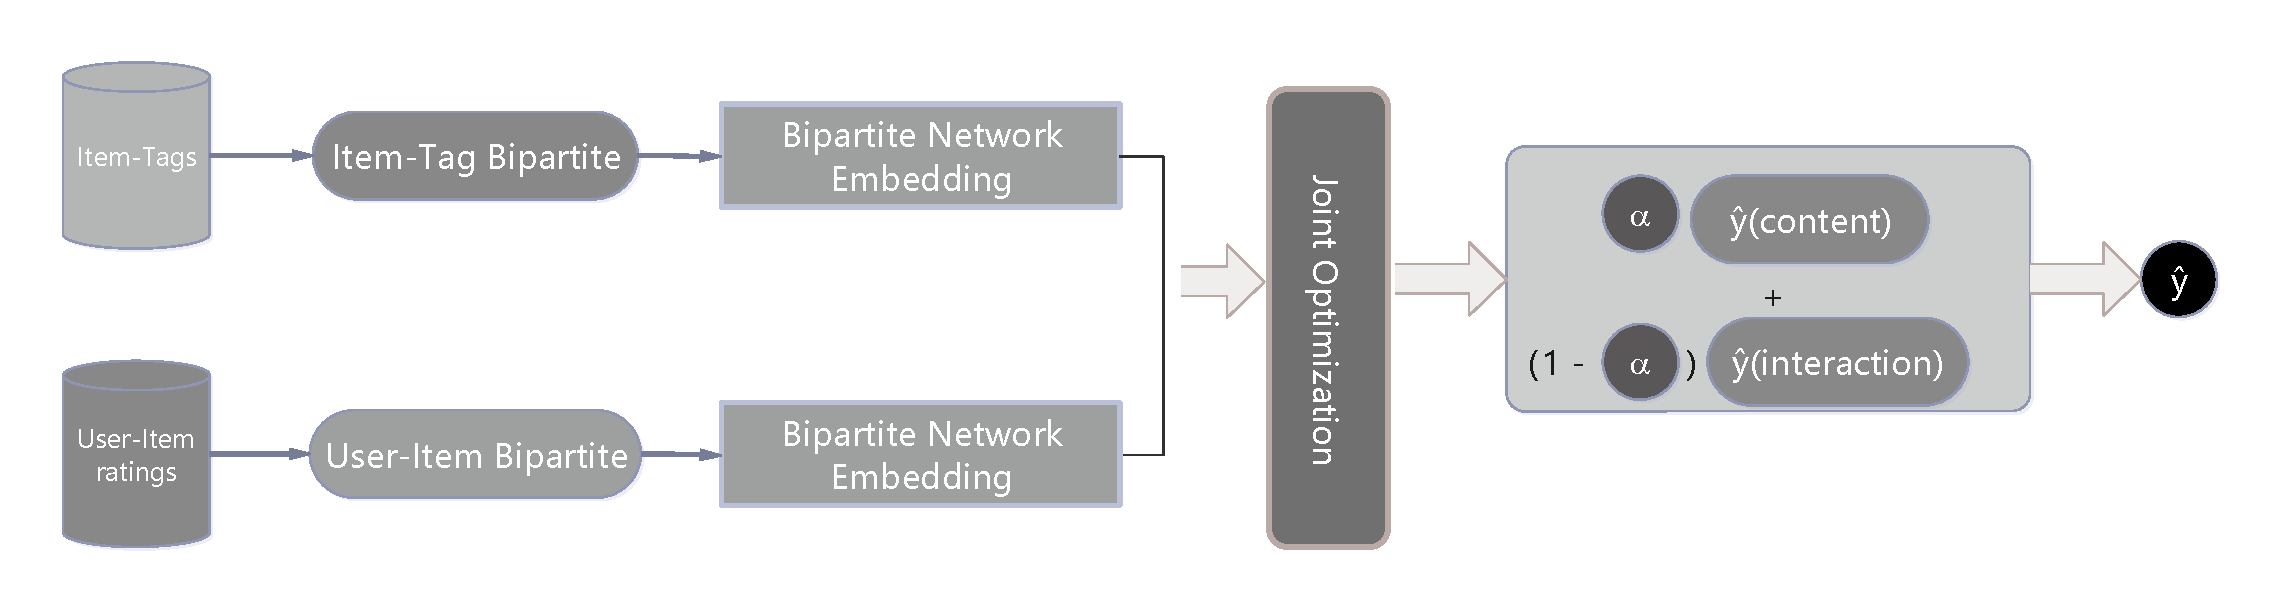
\includegraphics[width=1.0\textwidth]{imgs/framework.pdf}
	\caption{recommendation framework \label{fig:framwork}}
\end{figure}

\subsection{数据预处理}

这里介绍对数据进行的预处理,将user-item评分数据和item-tag内容数据表示成二部图。

\subsection{二部图嵌入表示}

这里介绍二部图的嵌入表示算法BiNE。


\subsection{联合训练}

这里介绍模型中联合训练用户和项目嵌入表示的算法。

\begin{equation}
\begin{array}{c}
\min l(R,U,V,{S_U},{S_V}) = \frac{1}{2}I{(R - (\alpha  {U^T}V{S_V} +  (1 - \alpha )({S_U} {U^T}V) ))^2}\\
+ \frac{{{\lambda _U}}}{2}||U||_F^2 + \frac{{{\lambda _V}}}{2}||V||_F^2
\end{array}
\end{equation}

\begin{equation}
S_{ik} = \frac{PCC(i,k)}{\sum_{k \in T(i)} PCC(i,k)}
\end{equation}



\section{实验}

在本节中,我们使用 MovieLens 数据集和 GoodBooks 数据集进行实验,比较了我们的模型和其他传统模型的实验效果,最后还分析了不同的参数设置对模型的影响。


\subsection{实验设置}

使用 MovieLens 数据集和 GoodBooks 数据集。

\subsection{性能评估}

这里比较

\begin{table}[tbp]
	\centering
	\caption{Prediction performance on MovieLens and GoodBooks \label{tab:result}}
	\setlength{\tabcolsep}{7mm}
	
	\begin{tabular}{ccrrrr}
		\toprule
		\multicolumn{ 2}{c}{Algorithm} & \multicolumn{ 2}{c}{MovieLens} & \multicolumn{ 2}{c}{GoodBooks} \\
		
		\multicolumn{ 2}{c}{} &       RMSE &        MAE &       RMSE &        MAE \\
		\midrule
		
		\multicolumn{ 2}{c}{User-CF} &     0.9335 &      0.725 &     1.1657 &     0.8209 \\
		
		\multicolumn{ 2}{c}{Item-CF} &     1.1425 &     0.8241 &     0.9559 &     0.7584 \\
		
		\multicolumn{ 2}{c}{MF} &     1.4479 &     1.0255 &     1.3978 &     0.9972 \\
		
		\multicolumn{ 2}{c}{User-NEMF} &     1.1534 &     0.8354 &     0.9529 &     0.7587 \\
		
		\multicolumn{ 2}{c}{Item-NEMF} &     0.9381 &     0.7294 &     0.9018 &     0.7081 \\
		
		\multicolumn{ 2}{c}{\textbf{NEMF}} &     \textbf{0.8657} &     \textbf{0.6636} &     \textbf{0.8684} &     \textbf{0.6804} \\
		\bottomrule
	\end{tabular} 	
\end{table}

\subsection{模型分析}

我们现在研究不同模型设置对模型的影响。

%\begin{figure}[htbp]
%	\centering
%	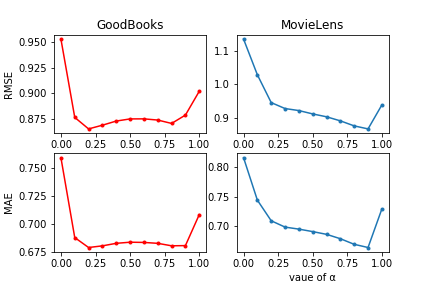
\includegraphics[width=0.8\textwidth]{imgs/alpha.png}
%	\caption{the inspect of Value $ \alpha $ \label{fig:alpha}}
%\end{figure}


\begin{figure}[htbp]
	\centering
	\subfigure{
		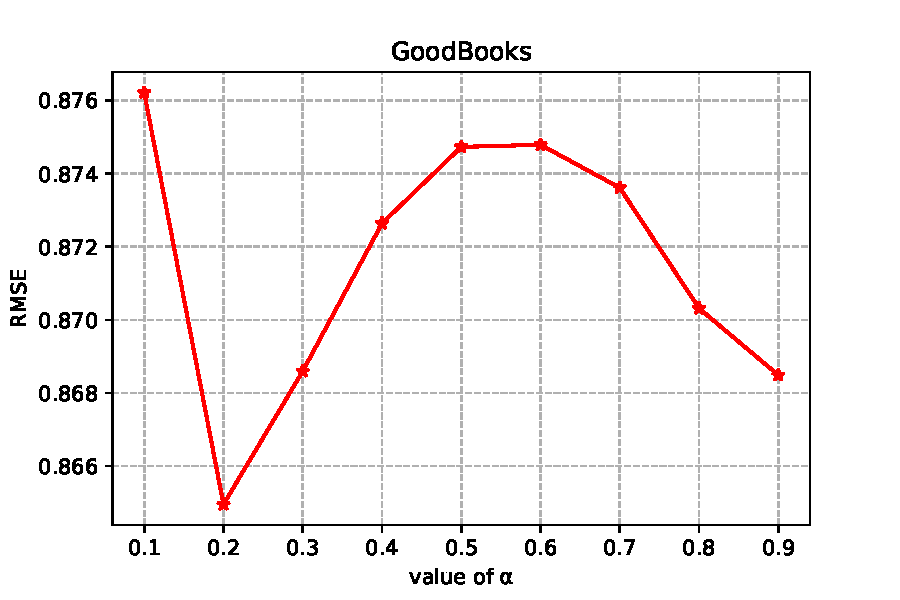
\includegraphics[width=0.4\textwidth]{imgs/alpha_1.pdf}
	}
	\quad
	\subfigure{
		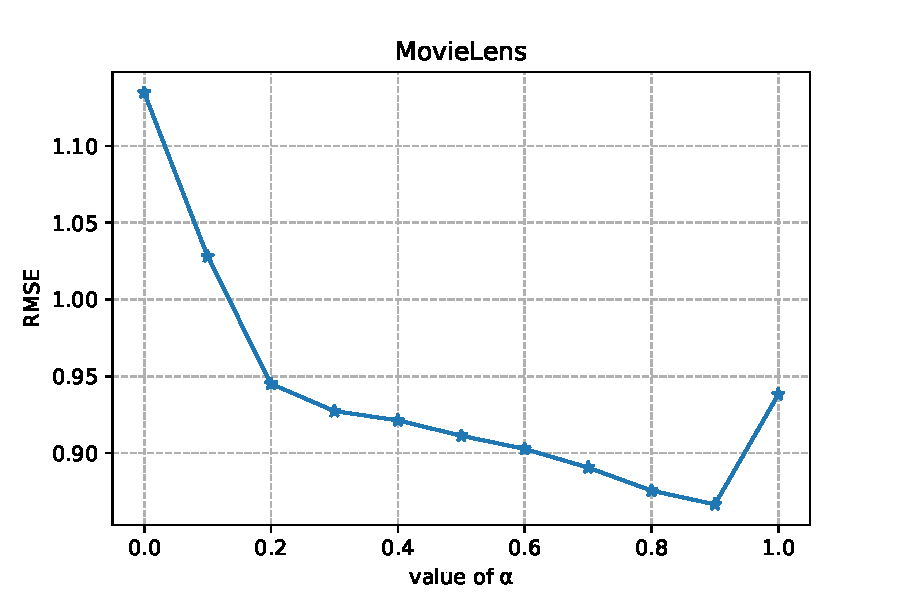
\includegraphics[width=0.4\textwidth]{imgs/alpha_2.pdf}
	}
	\quad
	\subfigure{
		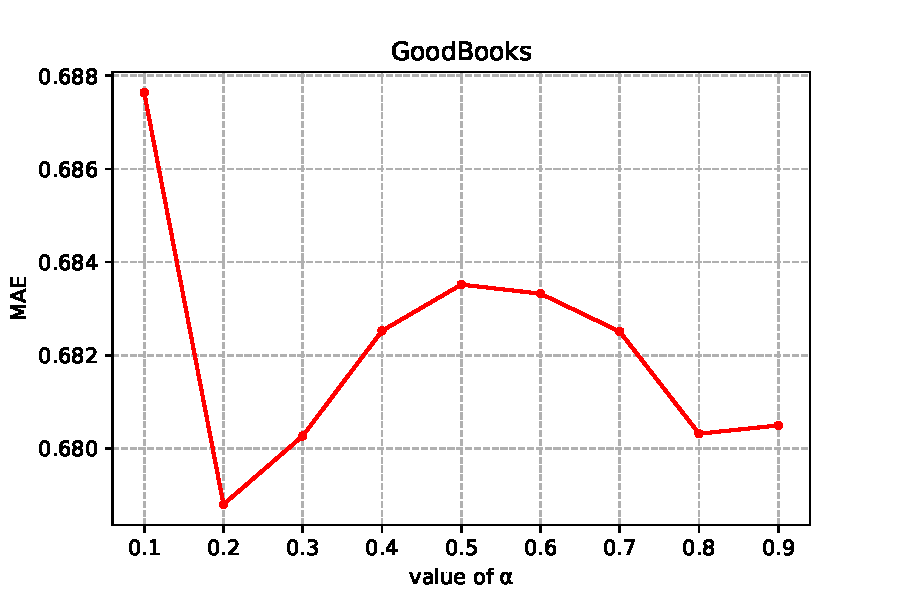
\includegraphics[width=0.4\textwidth]{imgs/alpha_3.pdf}
	}
	\quad
	\subfigure{
		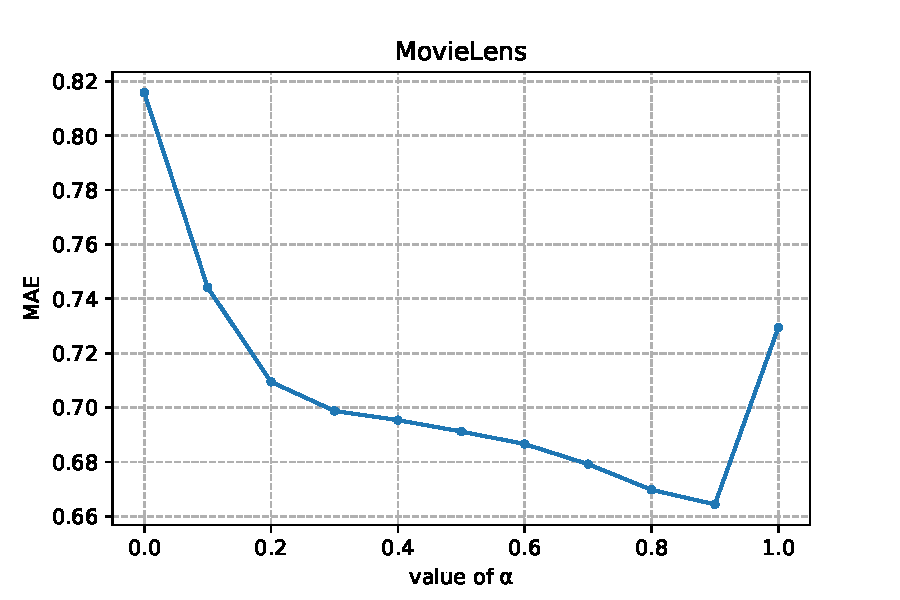
\includegraphics[width=0.4\textwidth]{imgs/alpha_4.pdf}
	}
	\caption{ the inspect of Value $ \alpha $\label{fig:alpha}} 
\end{figure}




\textbf{参数 $ \alpha $ 值的影响}。 研究$ \alpha $ 值对模型的影响。结果如图\ref{fig:alpha}

\textbf{阈值的影响}。 研究阈值对模型的影响。

\textbf{联合训练时矩阵维度的影响}。 联合训练时矩阵维度对模型的影响。


\section{结论}
结论部分,介绍论文的实验结果

% \nocite{*} 代表显示所有的论文文献 包括文中没有引用的

\bibliographystyle{unsrt}
\bibliography{wpref}

\end{document}
